Pingo ist eine Software-Lösung, die bereits seit dem Jahr 2011 an der Universität Paderborn entwickelt wird. Der Name ist ebenfalls ein Akronym und steht für „\textbf{P}eer \textbf{In}struction for Very Large \textbf{G}r\textbf{o}ups“. Im Gegensatz zu StuReSy ist Pingo bereits weiter verbreitet und wird an vielen deutschen Hochschulen eingesetzt (im September 2018 gab es 22.000 angemeldete Nutzer). Dahinter stand außerdem ein ganzes Team akademischer Mitarbeiter. Seit 2019 wird Pingo von der universitätsnahen Coactum GmbH betrieben und angeblich auch weiterentwickelt. Das Projekt ist damit deutlich kommerzieller und professioneller ausgerichtet als StuReSy.

Im Gegensatz zu StuReSy is Pingo in Bezug auf den Verbindungsaufbau und die Organisation von einzelnen Sitzungen etwas fortschrittlicher aufgebaut: Es handelt sich bei Pingo um eine reine Web-Applikation, die öffentlich unter \texttt{trypingo.com} auffindbar ist und kostenlos genutzt werden kann. Sowohl Administratoren als auch Teilnehmer können alle Arbeiten im Browser erledigen, ein Software-Download ist nicht notwendig. Für die administrative Nutzung muss jedoch ein Benutzerkonto erstellt werden. Einzelne Sitzungen werden durch numerische IDs im Namensraum eines Pingo-Servers identifiziert.


Pingo steht unter einer Open-Source-Lizenz und betreibt eine kostenlose Server-Instanz. Alternativ können Nutzer auch eine eigene Pingo-Server-Instanz betreiben. Pingo ist in der Programmiersprache Ruby und mithilfe des Web-Frameworks „Ruby on Rails“ implementiert worden. Entsprechend dazu muss ein potenzieller Server auch über einen Ruby-Interpreter und über eine NoSQL-Datenbank verfügen, um Pingo ausführen zu können.

In ihren Kernfunktionen sind sich Pingo und StuReSy sehr ähnlich. Pingo hat jedoch insgesamt den größeren Funktionsumfang. Trotzdem fehlen entscheidende Funktionen für den Einsatz in der Programmierlehre:
\begin{itemize}
    \item \textbf{Keinerlei Formatierungs-Möglichkeiten}: Fragen innerhalb der Pingo-Plattform können nicht formatiert werden. Damit können selbst simple Formatierungen wie Fettschreibungen, Unterstreichungen oder Zeilenumbrüche nicht verwendet werden. Dementsprechend ist auch die übersichtliche Darstellung von Quelltext unmöglich und Pingo für den Einsatz in der Programmierlehre gänzlich ungeeignet.
\end{itemize}

\begin{figure}[H]
    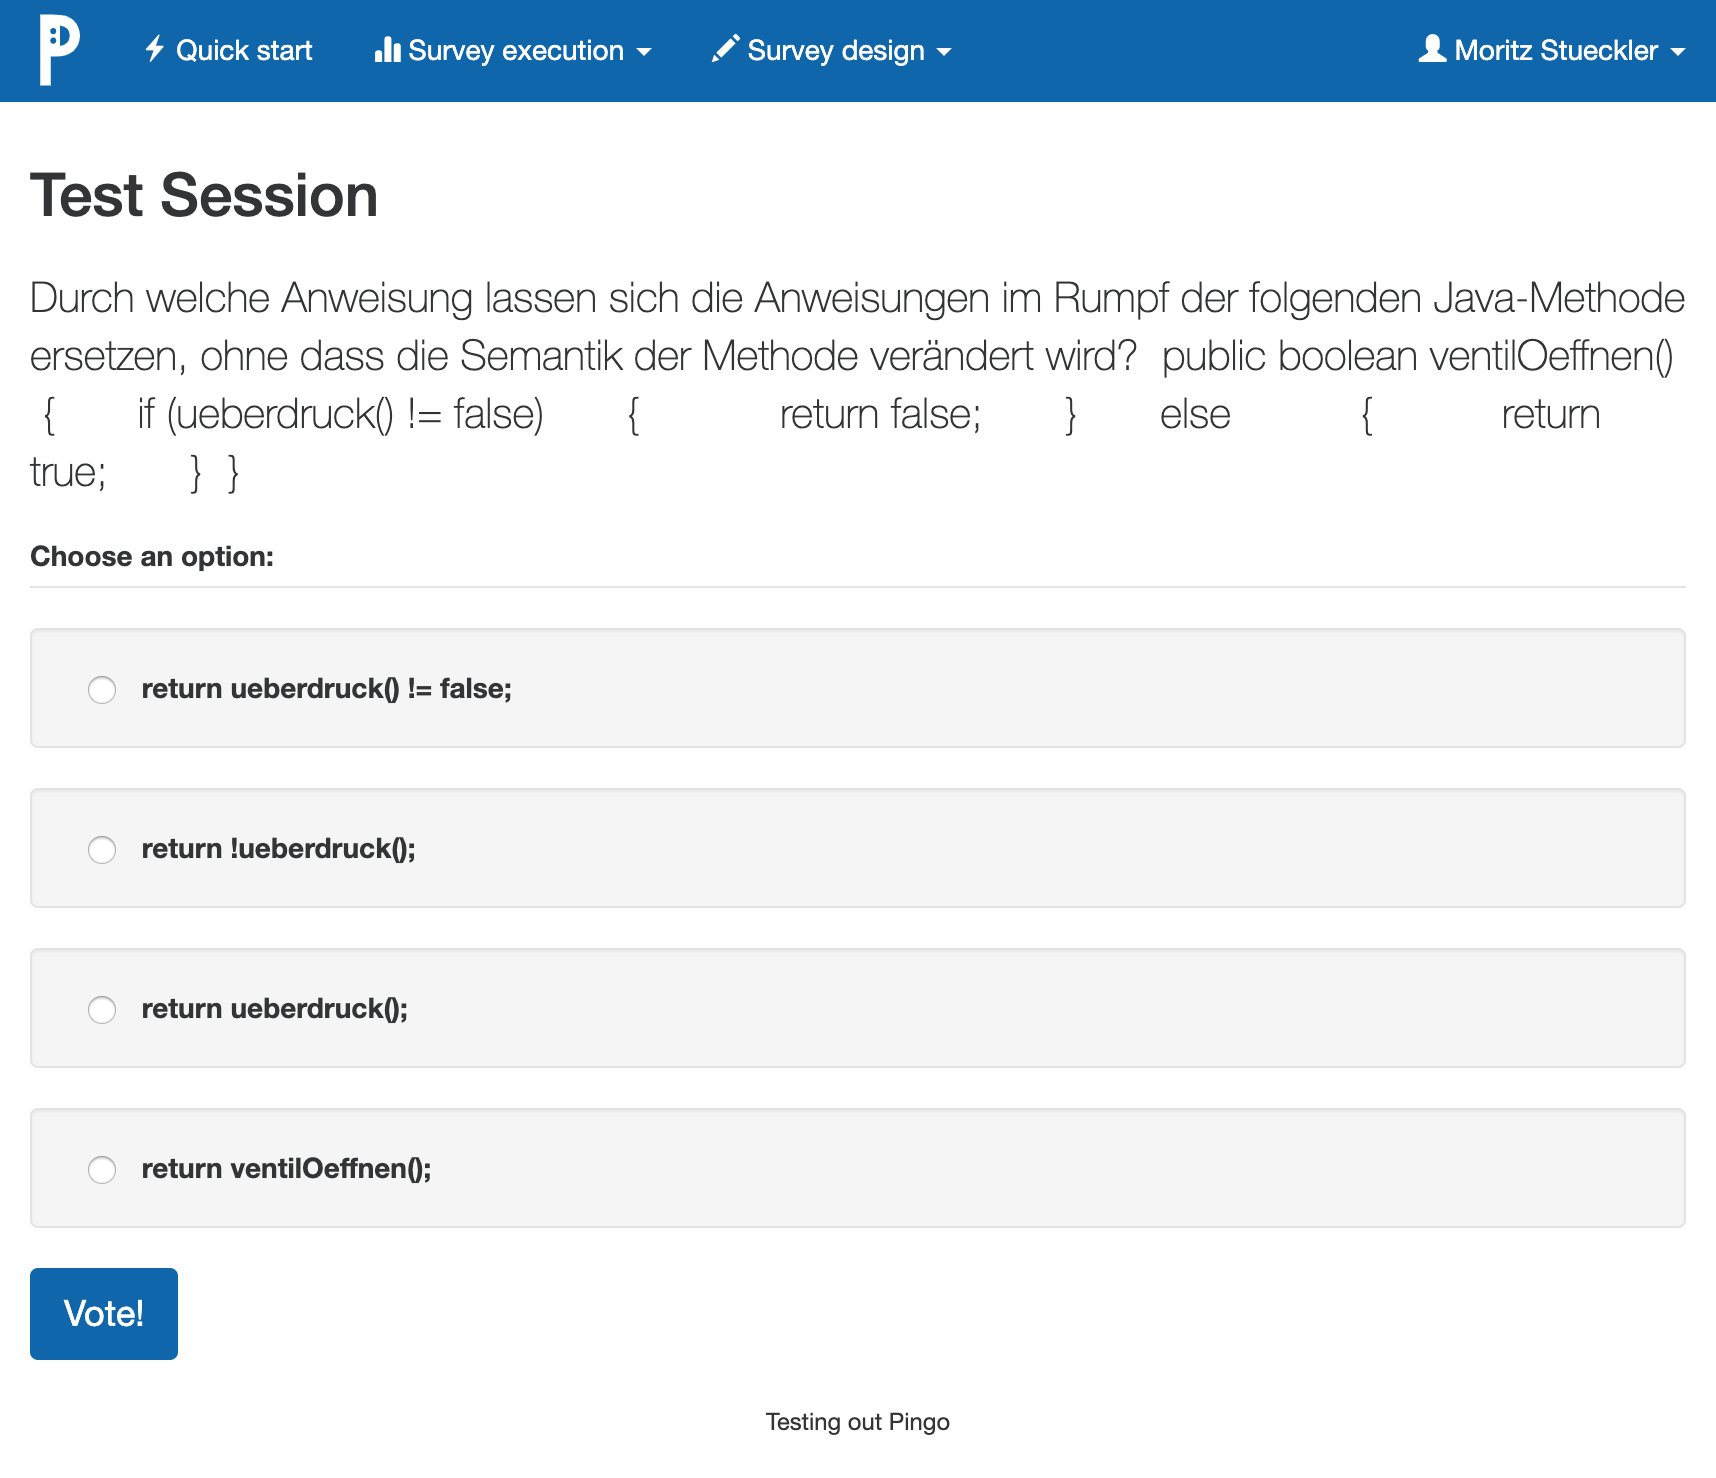
\includegraphics[width=12cm]{chapter/bewertung/bilder/pingo_problem1.png}
    \centering
    \caption{Pingo verfügt über keinerlei Text-Formatierungsoptionen und ist daher ungeeignet für die Darstellung von Quelltext.}
    \label{abb:pingo_frage}
\end{figure}